\documentclass[12pt,a4paper]{article}
\usepackage[utf8]{inputenc}
\usepackage[german]{babel}
\usepackage[T1]{fontenc}
\usepackage{amsmath}
\usepackage{amsfonts}
\usepackage{amssymb}
\usepackage{graphicx}
\usepackage{siunitx}
\usepackage{float}
\usepackage[left=2cm,right=2cm,top=2cm,bottom=2cm]{geometry}
\author{Gerald}

\begin{document}
\sisetup{separate-uncertainty = true}
	\setlength{\parindent}{0pt} 
	\begin{center}
		{\LARGE Versuchsprotokoll}\\
		\begin{large}
			zum Fortgeschrittenenpraktikum im Bachelorstudiengang Physik\\[0.4cm]
			an der RWTH Aachen\\
			II. Physikalisches Institut A\\[5.5cm]
			\Large\textbf{\textsl{Gasdetektoren und Statistik (T07)}}\\[5.5cm]
			\normalsize\textit{vorgelegt\\von}\\[0.4cm]
			\large{Moritz Berger (355244)\\Gerald Kolter (355005)}\\\textbf{Gruppe 30}\\[2cm]
			\large \textbf{Wintersemester 2017/18}
		\end{large}
	\end{center}
	\newpage
	
	\tableofcontents
	\newpage
	
	
\section{Versuchsziel}
Das Ziel dieses Versuches ist in zwei Teile aufgeteilt.\\
Als erstes sollen die Eigenschaften eines Proportionalzählers und eines Geiger-Müller-Zählrohres untersucht werden. Dazu wird zum einen die Charakteristik, also die Abhängigkeit der Zählrate von der angelegten Spannung, untersucht, um den optimalen Bereich für die Betriebsspannung zu erhalten. Es wird außerdem die Abhängigkeit der Stärke eines Pulses des Proportionalzählers von der Spannung betrachtet und die Tot- und  Erhohlungszeit des Geiger-Müller-Zählers bestimmt.\\
Im zweiten Versuchsteil sollen Messungen zur Statistik durchgeführt werden, die verschiedene vorhergesagte Verteilungen bestätigen. Dabei soll eine Gaussverteilung für eine hohe Anzahl an Messungen, eine Poissonverteilung für kleine Messergebnisse und eine Exponetialverteilung für den Abstand zwischen zwei gemessenen Zerfällen untersucht werden. 

\section{Funktion}
Ein Geiger Müller Zählrohr besteht aus einer mit einem Gasgemisch gefüllten Kammer. Beim Durchgang von Strahlung entstehen in dieser Kammer Elektron-Ionen Paare. Durch eine  Hochspannungsquelle wird nun zwischen der Wand der Kammer und einem sich in der Mitte befindenden Drahtes eine Hochspannung angelegt. Dadurch verhindert man die Rekombination der Ionen und erzeugt durch Gasverstärkung weitere Paare, wodurch ein messbarer Puls entsteht.\\
Die zum Draht wandernden Elektronen schirmen allerdings das durch die Spannung erzeugte Elektrische Feld ab, wodurch für einen Zeitraum keine neuen Pulse gemessen werden können. Daduruch entsteht eine Totzeit.\\
Die zur Außenwand wandernden Ionen bewirken ebenfalls eine Abschwächung des E-Feldes, wodurch gemessene Pulse kurz nach der Totzeit weniger verstärkt werden und deswegen kleiner sind. Die Zeit bis zum erreichen der originalen Pulshöhe nennt man Erholungszeit.\\
Die Auslösezeit gibt an, nach welcher Zeit im Messaufbau wieder ein Puls gemessen werden kann.\\
\\
Ein Proportionalzählrohr funktioniert ähnlich, nur das durch eine kleinere angelegte Spannung die Gasverstärkung kontrollierter abläuft und dadurch ein Zusammenhang zwischen Energie des auslösenden Teilchens und der Pulshöhe besteht.\\
Außerdem ist durch den kleineren Puls die Totzeit um ein vielfaches kleiner, sodass sie nicht berücksichtigt werden muss.\\
\\
Beide Zählrohre besitzen eine Charakteristik, die das Verhalten der gezählten Pulsrate in Abhängigkeit von der angelegten Spannung beschreibt. In diesen gibt es Bereiche, sogenannte Plateaus, in denen die Zählrate nahezu konstant ist. Diese Bereiche eignen sich am besten für eine Messung.

\section{Aufbau}
\subsection{Geiger-Müller-Zählrohr}
Der Aufbau des Geiger Müller Zährohres besteht aus einer Probenkammer, an die das Zählrohr befestigt ist. In diese Kammer kann man das Präparat legen. An das Zählrohr ist eine Hochspannungsquelle angeschlossen, mit der man eine Hochspannung von maximal 700V an das Zählrohr anlegt.\\
Die gemessenen Zählpulse werden durch einen Verstärker verstärkt und sowohl an ein Oszilloskop, das den Spannungsabfalls misst, welcher proportional zur Pulshöhe ist, als auch an ein Zählgerät, das die Anzahl der in einer bestimmten Zeit ankommenden Pulse zählt, weitergeleitet.\\
Vor dieses Zählgerät kann noch eine Totzeitstufe geschaltet werden.
\subsection{Proportionalzähler}
Der Aufbau des Proportionalzähler ist ähnlich zum Geiger-Müller-Zählrohr. Es wird hier ein Durchflusszähler verwendet, durch den ein Argon-Methan-Gasgemisch geleitet wird. Die Probe kann durch einen Drehteller direkt in das Zählrohr gebracht werden. Auch hier wird das gemessene Signal durch einen Verstärker verstärkt und an ein Oszilloskop und ein Pulszähler weitergeleitet.
\section{Durchführung}
\subsection{Geiger-Müller-Zählrohr}
Alle Messungen zum Geiger-Müller-Zählrohr werden mit dem $_{38}^{90}Sr$-Präparat durchgeführt. Dieses sendet $\beta$-Strahlung der Energien 0.546MeV und 2.28MeV aus\footnote{Quelle: http://www.periodensystem-online.de}.
\subsubsection{Charakteristik}
Die Charakteristik wird gemessen, indem bei eingebrachtem Präparat die Spannung, ausgehend von der Minimaleinstellung von \SI{250}{V}, in \SI{10}{V} Schritten erhöht und jeweils über \SI{10}{s} die Anzahl der gemessenen Ereignisse erfasst wird.\\
Um die Einsatzspannung $U_E$ und die Geiger-Schwelle $U_G$ genauer bestimmen zu können wurde im entsprechenden Bereich, in dem sich diese Werte befinden, in \SI{2}{V} Schritten statt in \SI{10}{V} Schritten gemessen.\\
\\Eine Schnellauswertung ergab $U_G = \SI{350}{V}$. Um sicher zu gehen, dass das Zählrohr für die folgenden Messungen im richtigen Spannungsbereich arbeitetet, wird die Spannung auf $U = U_G + 100V = \SI{450}{V}$ eingestellt.

\subsubsection{Untergrundrauschen}
Um eine mögliche Störung durch Untergrundrauschen zu beseitigen, wurde mit einer leeren Kammer insgesamt 5 mal über $\SI{1}{min}$ die Pulsrate gemessen.

\subsubsection{Totzeit}
Zur Totzeit des Geiger-Müller-Zählrohres sollen zwei verschiedene Messungen gemacht werden.
\paragraph{Stever-Diagramm}
Als erstes wird ein Stever-Diagramm erstellt, an dem man die Tod- und Erholungszeit ablesen kann. Dazu wird auf dem Oszilloskop ein unendliches Nachleuchten eingestellt. Der Trigger sollte dabei niedrig genug eingestellt sein, um möglichst alle Pulse zu erkennen. Er wurde bei einer maximal gemessenen Spannung von c.a 300mV auf 10mV gestellt. Durch die richtige Wahl der Zeitskala in der Größenordnung von einigen \SI{100}{\mu s} sollte die Einhüllender der Erholungszeit sichtbar werden. Hier wurde einmal eine Zeitskala von \SI{100}{\mu s} und eine von \SI{250}{\mu s} ausgewählt. Anhand der Einhüllenden wird nun händisch die Tot- und Erholungszeit abgelesen. Dabei befindet sich die Totzeit beim Nulldurchgang der Einhüllenden und die Erholungszeit beim Erreichen der Ausgangspulsgröße. 

\paragraph{Totzeitkorrektur}
Als zweites wird die Auflösungszeit mithilfe einer Totzeitstufe bestimmt. Mithilfe dieser kann man eine Totzeitkorrektur der gemessenen Zählraten durchführen. Dabei ist die wirkliche Zählrate N in Abhängigkeit von der gemessenen Rate n und der Auflösungszeit $\tau$ gegeben durch 
\begin{equation}
\label{Totzeitkorrektur}
N = \dfrac{n}{1-n\tau}
\end{equation}
Nun werden für zwei verschiedene künstlich angelegte Totzeiten $\tau_{2ms}$ und $\tau_{1\mu s}$ die Zählrate bestimmt.\\Dazu werden zuerst die Frequenzen der Totzeitstufe überprüft, um sicher zu stellen, dass diese richtig kalibriert ist. Dafür wird mithilfe eines Frequenzgenerators eine 1MHz Frequenz an die Totzeitstufe angelegt und über 1s die Anzahl der durchgelassenen Pulse gemessen.\\
Danach werden die beiden Zählraten bestimmt. Dazu wird für beide Zeiten 1 Minute lang die Zählrate gemessen. Da N für beide Totzeiten gleich sein sollte und $\tau_{1\mu s} << \tau$ gilt, kann man durch Gleichsetzten von Gleichung \ref{Totzeitkorrektur} für beide Zeiten die Auflösungszeit bestimmen:
\begin{equation}
\tau_{1\mu s} \approx \tau = \dfrac{1}{n_{1\mu s}} - \dfrac{1}{n_{2ms}} + \tau_{2ms}
\label{Auslosungszeit}
\end{equation}

Die Messung wurde zuerst mit der Probe auf der mittleren Schiene durchgeführt, und dann mit der Probe auf der 2. Schiene von oben insgesamt 3 mal wiederholt, damit die Zählrate hoch genug ist und die Messung genauer wird.
\subsection{Proportionalzähler}

\subsubsection{Charakteristik}
Beim Proportionalzähler wurde ebenfalls die Charakteristik vermessen, und zwar einmal Anhand der $_{95}^{241}Am$-Probe und einmal anhand der $_6^{14}C$-Probe. \\
Das Am-Präparat sendet dabei $\alpha$-Strahlung von c.a 5MeV und $\beta$-Strahlung von 0.57MeV aus.\\
Das C-Präparat sendet $\beta$-Strahlung von 0.16MeV aus\footnote{Quelle: http://www.periodensystem-online.de}.\\
Dazu wurde in \SI{20}{V} oder (aus Zeitgründen) in \SI{40}{V} Schritten, wieder ausgehend von \SI{250}{V}, jeweils über \SI{10}{s} die Pulsrate aufgenommen. Bei \SI{1200}{V} musste die Hochspannungsquelle auf 2 fache Verstärkung umgestellt werden. Es kann sein, dass die in Wirklichkeit angelegte Spannung für die beiden Verstärkungsmodi nicht gleich ist, was sich auf die Messdaten auswirken kann.\\
Außerdem wurde eine Untergrundmessung mit leerem Probenraum für den vollständigen untersuchten Spannungsbereich durchgeführt.

\subsubsection{Pulshöhe}
Da beim Proportionalzähler die Pulsstärke abhängig von der Energie der Teilchen ist, wurde zusätzlich noch die Pulshöhe mithilfe des Oszilloskopes für alle Spannungswerte bestimmt.  Dies geschieht, indem auf dem Oszilloskop die ungefähre Mittlere Höhe der ankommenden Pulse abgelesen wird.

\subsection{Statistikmessung}
Die Statistikmessungen wurden alle mit dem Geiger-Müller-Zählrohr, und damit auch mit dem Sr-Präparat, aufgenommen.
\subsubsection{Poissonverteilung}
Die Zerfälle sind poissonverteilt. Um eine Poissonverteilung auch in den Messdaten beobachten zu können, muss die Messzeit klein gehalten werden (T = 0.3s), da die Verteilung ansonsten in eine Gaußverteilung übergeht. Die Poissonverteilung ist nur für diskrete Werte definiert und hat die Form:
\begin{equation}
P(n) = \dfrac{\mu ^n}{n!} \cdot e^{-\mu}
\end{equation}
\subsubsection{Gaußverteilung}
Da die Zerfälle poissonverteilt sind, muss für die Messung einer Gaußverteilung die Messzeit um Faktor 10 erhöht werden (T = 3s). Die Gaußverteilung hat die Form:
\begin{equation}
P(x) = \dfrac{1}{\sqrt{2 \pi} \sigma} \cdot e^{\frac{(x - \mu)^2}{2 \cdot \sigma ^2}}
\end{equation}
\subsubsection{Exponentialverteilung}
Die Abstände zwischen zwei Zerfällen sind exponentialverteilt. Zur Messung werden mit dem Oszilloskop Bilder gemacht, auf denen mehrere Zerfälle zu sehen sind. Die Exponentialverteilung hat die Form:
\begin{equation}
P(\Delta t) = A \cdot e^{- A \Delta t}
\end{equation}
\newpage
\section{Ergebnisse}
\subsection{Geiger-Müller-Zählrohr}

\subsubsection{Totzeit mithilfe des Stever-Diagramms}

\begin{figure}
\centering
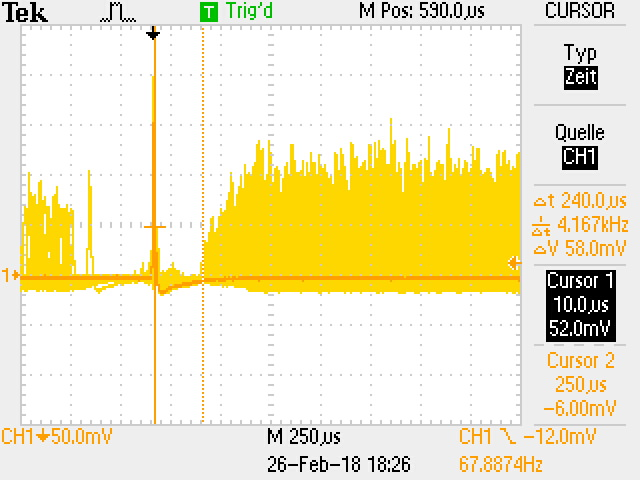
\includegraphics[scale=0.49]{Bilder/Stever/Stever1_1.PNG}
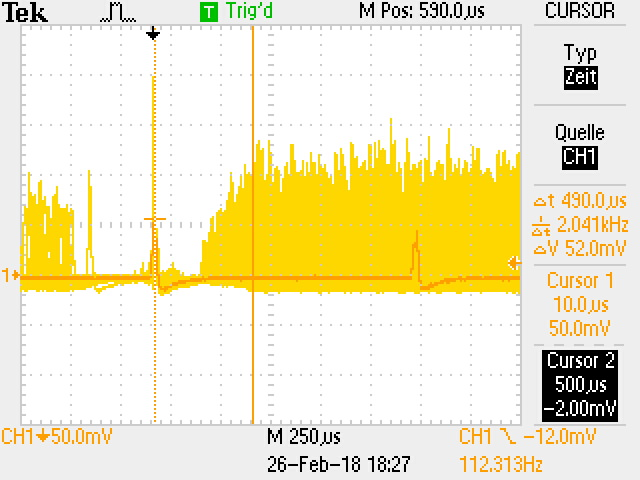
\includegraphics[scale=0.49]{Bilder/Stever/Stever1_2.PNG}
\caption{Stever-Diagramm mit einer Zeitauflösung von 250$\mu s$. Im linken Bild wurde mit dem Cursor der ungefähre Nulldurchgang zur Bestimmung der Totzeit angepeilt, im rechten Bild der Punkt, in dem die anfängliche Peakhöhe wieder erreicht wurde, woraus die Erholungszeit ermittelt wurde. Die Werte wurden bei der Auswertung nachkorrigiert}
\label{fig:Stever}
\end{figure}

\begin{figure}
\centering
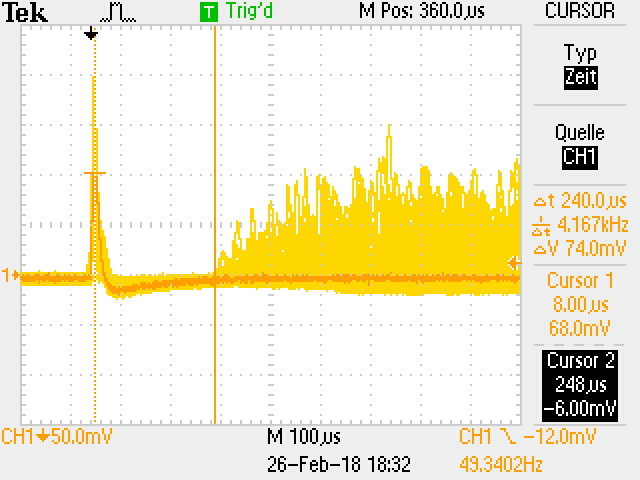
\includegraphics[scale=0.49]{Bilder/Stever/Stever2_1.PNG}
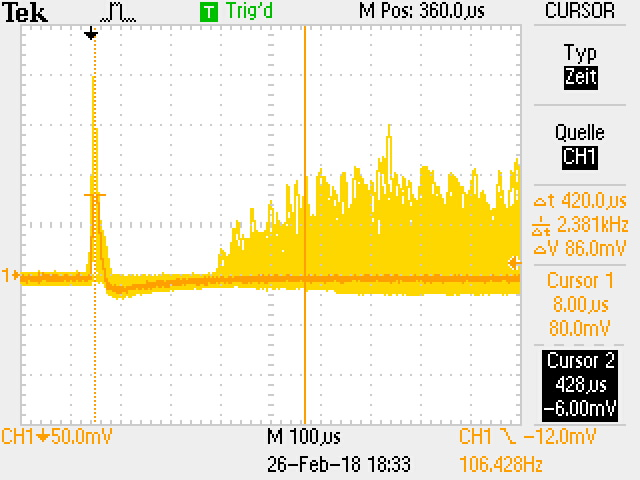
\includegraphics[scale=0.49]{Bilder/Stever/Stever2_2.PNG}
\caption{Stever-Diagramm mit einer Zeitauflösung von 100$\mu s$. Das linke Bild dient wieder zur Abschätzung der Totzeit, das rechte zur Abschätzung der Erholungszeit.}
\label{fig:Stever2}
\end{figure}


In Abbildung \ref{fig:Stever} und \ref{fig:Stever2} sind die Oszilloskopbilder für zwei unterschiedliche Zeitskalen mit jeweils den ersten Abschätzungen für die Tot- und Erholungszeiten dargestellt. An der größeren Zeitskala kann man die Totzeit nicht so genau ablesen wie bei der kleineren, allerdings ist die Einhüllende besser zu erkennen, wodurch die Bestimmung der Erholungszeit einfacherer ist. Deswegen wurden beide Messreihen für die Auswertung benutzt.
Leider konnten die Daten nicht aus dem Oszilloskop extrahiert werden, da das Nachleuchten nicht mit abgespeichert wurde, weswegen die Auswertung vollständig visuell gemacht werden muss.\\
\\
Die Totzeit wird anhand der linken Grenze der Einhüllenden bestimmt. Da durch die eingestellte Schwelle des Verstärkers zu kleine Pulse nicht registriert werden, ist die echte Totzeit etwas kleiner als die abgelesene Grenze.\\
Die Erholungszeit wird bestimmt, indem der Punkt abgelesen wird, ab dem die Peakhöhe einen konstanten Wert annimmt.
Sie kann man nicht so genau bestimmt werden, da durch die große statistische Schwankung der Peaks nicht genau erkennbar ist, an welchem Punkt diese Bedingung erreicht ist.\\
Die abgelesenen Ergebnisse sind in Tabelle \ref{teb:Stever} aufgelistet. Die Fehler wurden durch die Ableseungenauigkeit abgeschätzt.

\begin{table}[H]
\centering
\begin{tabular}{|c|c|c|}
\hline
Zeitskala$[\mu s]$ & Totzeit$[\mu s]$ & Erholungszeit$[\mu s]$\\
\hline 
250 & $220\pm 20$ & $520\pm 50$ \\
\hline 
100 & $220\pm 10$ & $450\pm 30$ \\
\hline
\end{tabular}
\caption{Ergebnisse der Totzeitbestimmung an beiden Zeitskalen. }
\label{teb:Stever}
\end{table}

Eine gewichtete Mittelung ergibt (mit äußerem Fehler):

\begin{equation}
\boxed{T_D = \SI{220 \pm 9}{\mu s}}
\end{equation}

\begin{equation}
\boxed{T_R = \SI{469 \pm 31}{\mu s}}
\end{equation}

\subsubsection{Auslösezeit mithilfe der Totzeitstufe}


\paragraph{Kalibration}
Vor der eigentlichen Messung mit der Totzeitstufe wurde eine Kalibration durchgeführt. Die Ergebnisse sind in Tabelle \ref{tab:Totzeitkalibration} aufgelistet. Die Messung wurde mehrfach wiederholt, um sicher zu stellen, dass das Ergebnis exakt ist. Es ergab sich mehrfach derselbe Wert, weswegen das Ergebnis auf $1\mu s$ exakt angenommen werden kann. Relevant für die weitere Auswertung ist nur die $2ms$ Stufe, die auf $1.908ms$ kalibriert wurde.

\begin{table}[H]
\centering
\begin{tabular}{|c|c||c|}
\hline
Einstellung & $1\mu$ s & $2ms$\\
\hline 
Pulsrate & $1000003$ & $524$ \\
\hline 
Auslösezeit & $1\mu s$ & $1.908ms$ \\
\hline
\end{tabular}
\caption{Ergebnisse der Kalibration der Totzeitstufe. Es ist die gemessene Pulsrate über 1s und die daraus berechnete Auslösezeit angegeben.}
\label{tab:Totzeitkalibration}
\end{table}

\paragraph{Bestimmung von der Auslösezeit $\tau$}



In Tabelle \ref{tab:Totzeitstufe} sind die Ergebnisse der Messungen zur Totzeitstufe aufgelistet. Der Fehler wurde mit $\sqrt{N}$ angenommen.\\
Daraus wurde mithilfe von Gleichung \ref{Totzeitkorrektur} die Auflösezeit bestimmt, welche ebenfalls in der Tabelle aufgelistet ist. Der Fehler wurde folgendermaßen errechnet:

\begin{equation}
\sigma_{\tau} = \sqrt{\left(\dfrac{\sigma_{n_{1\mu s}}}{n_{1\mu s}^{2}}\right)^2 + \left(\dfrac{\sigma_{n_{2ms}}}{n_{2ms}^{2}}\right)^2}
\end{equation}

Diese Methode ist extrem anfällig auf Änderungen in der Zählrate, da durch die Addition von $T_{2ms}$ das Ergebnis um eine ganze Größenordung (im Betrag) kleiner wird, als wenn man dies weglassen würde. Da der Fehler sich dabei aber nicht ändert, reicht bereits eine Änderung in den Zählraten von $1\%$, um das Ergebnis signifikant zu verschieben.\\
\\
Durch eine gewichtete Mittelung der Ergebnisse kann der Fehler noch etwas verbessert werden.\\
Dies führt zu einem Endergebnis von:
\begin{equation}
\boxed{\tau = \SI{318\pm 56}{\mu s}}
\end{equation}
Dieser Wert liegt zwischen der bestimmten Totzeit und der Auslösezeit.
In Abbildung \ref{fig:Totzeit} ist die Auswirkung der Totzeitkorrektur mithilfe von Gleichung \ref{Totzeitkorrektur} dargestellt.

\begin{figure}
\centering
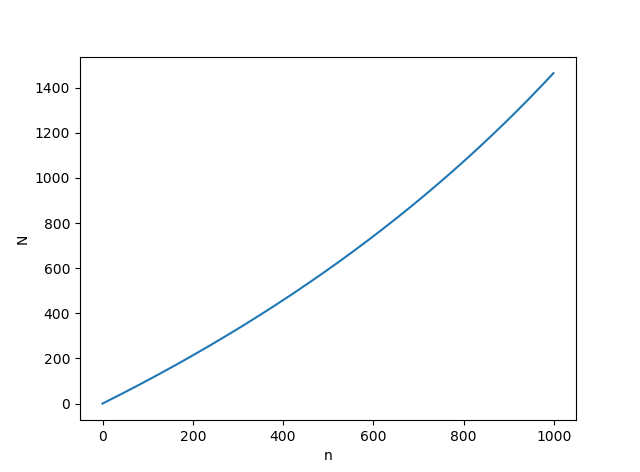
\includegraphics[scale=0.9]{Bilder/Totzeitkorrektur.png}
\caption{Auftragung der von der Totzeit bereinigten Zählrate N gegen die gemessene Zählrate n bei einer Auslösezeit von $318\mu s$.}
\label{fig:Totzeit}
\end{figure}

\begin{table}[H]
\centering
\begin{tabular}{|c|c|c|c|}
\hline
Messzeit[s] & 60 &60&60\\
\hline 
$N_{1\mu s}(gesamt)$ & $10603 \pm 103$ & $10689\pm 103$ & $10546\pm 103$ \\
\hline 
$N_{2ms}(gesamt)$ & $8284\pm 91$ & $8257 \pm 91$ & $8307\pm 91$ \\
\hline 
$n_{1\mu s}(Sekunde)$ & $176.7 \pm 1.7$ & $178.2 \pm 1.7$ & $175.8\pm 1.7$ \\
\hline 
$n_{2ms}(Sekunde)$ & $138.1\pm 1.5$ & $137.6 \pm 1.5$ & $138.5\pm 1.5$ \\
\hline 
$\tau [\mu s]$ & $324\pm 97 $ & $255 \pm 97$ & $375\pm 97$ \\
\hline
\end{tabular}
\caption{Ergebnisse der Messung mithilfe der Totzeitstufe. Angegeben sind jeweils für beide Totzeiten die gemessenen Zählraten über die ganze Messzeit, die auf eine Sekunde normierten Zählraten und die daraus bestimmte Auslösezeit.}
\label{tab:Totzeitstufe}
\end{table}


\subsubsection{Charakteristik}
\label{GMchar}

Die Ergebnisse wurden mithilfe der Rauschmessung vom Offset des Untergrundrauschens bereinigt. 
Außerdem wurde mithlife von Gleichung \ref{Auslosungszeit} die Totzeitkorrektur durchgeführt. In Abbildung \ref{fig:GMTotzeit} ist die Auswirkung dieser Korrekturen zu sehen.

\begin{figure}
\centering
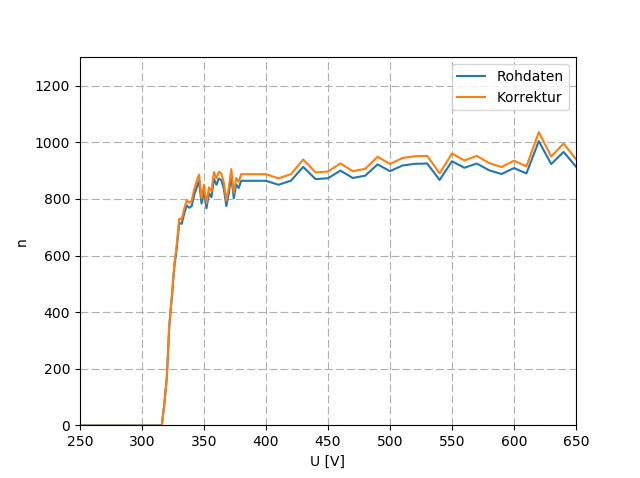
\includegraphics[scale=0.9]{Bilder/GMTotzeit.PNG}
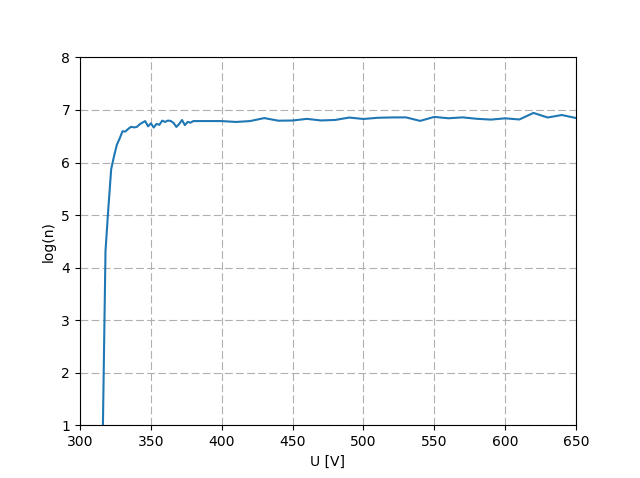
\includegraphics[scale=0.9]{Bilder/GMlogroh.PNG}
\caption{\textbf{Oberes Bild:} Auswirkungen der Offset- und Totzeitkorrektur. Die blauen Daten stellen die Orginalmessung dar, der orangene Plot die korrigierten Daten. \textbf{Unteres Bild:} Darstellung der lorarythmisierten Daten}
\label{fig:GMTotzeit}
\end{figure}

Mit zunehmender Spannung steigt die Messrate exponentiell, da immer mehr Ereignisse mit kleineren Energien registriert werden. Daher Müssen die Daten noch logarythmisiert werden, um das Plateau erkennen zu können. Dies ist ebenfalls in Abbildung \ref{fig:GMTotzeit} zu sehen.\\
Der relativ große Fehler auf die Totzeit ist dabei von systematischer Natur, er verschiebt also die Werte in die gleiche Richtung. Da das Plateau in der logarythmischen Sklaierung eben ist, verschiebt er die Werte um nahezu den gleichen Faktor, womit sich die Position der Einsatz- und Geiger-Spannung nicht nennenswert ändert. Der Fehler kann also für die Bestimmung dieser vernachlässigt werden.

\paragraph{Bestimmung der Geiger-Spannung}
\begin{figure}
\centering
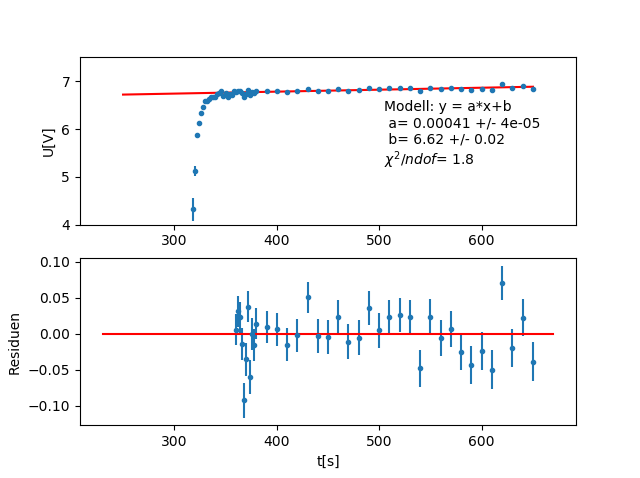
\includegraphics[scale=0.9]{Bilder/GMGeradenfit.PNG}
\caption{Fit der Geraden an das Plateau}
\label{fig:GMGeradenfit}
\end{figure}

\begin{figure}
\centering
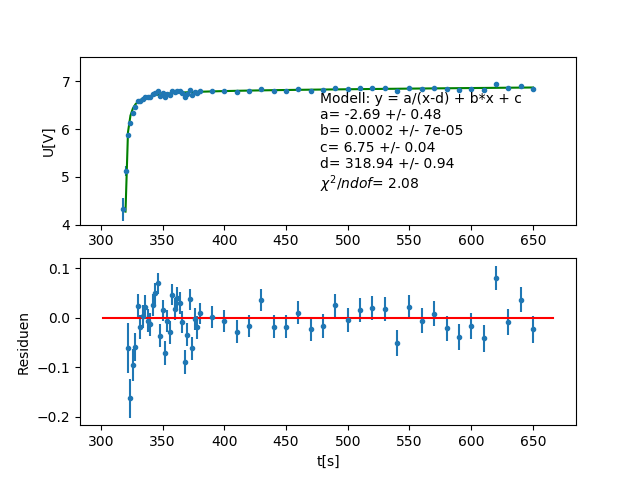
\includegraphics[scale=0.9]{Bilder/GMKurvenfit.PNG}
\caption{1/x-Fit an die Daten.}
\label{fig:GMKurvenfit}
\end{figure}

Anhand der logarythmisierten Daten wird nun die Geiger-Spannung $U_G$ bestimmt. Dazu  wurde als erstes abgeschätzt, dass das Plateau spätestens bei $\SI{360}{V}$ erreicht wird und ein Geradenfit an die Daten überhalb dieser Spannung angepasst. Dieser ist in Abbildung \ref{fig:GMGeradenfit} zu sehen.\\
Um nun den Anfang des Plateaus nicht nur über eine visuelle Abschätzung bestimmen zu können, wird außerdem noch ein Fit der Form
\begin{equation*}
y = \dfrac{a}{x+d} + b\cdot x + c
\end{equation*}
an die Daten angefitted. Es wurde hier eine $\dfrac{1}{x}$ Funktion gewählt, da es wegen der wenigen Datenpunkte, die groß von der Plateaugeraden abweichen, sehr schwierig gewesen ist eine Funktion an die Daten anzupassen und diese Funktion die einzige ist, bei der der Fit geglückt ist und die Umgebung der Geigerfrequenz gut beschreibt. Das Ergebnis ist in Abbildung \ref{fig:GMKurvenfit} dargestellt.\\
$U_G$ wird bestimmt, indem die Spannung gesucht wird, ab der die beiden Anpassungen innerhalb ihrer Unsicherheiten überseinstimmen. Es muss aber beachtet werden, dass die Anpassungen korrelieren, da sie aus demselben Datensatz stammen. Der Einfachheit halber wird angenommen, dass der Fehler des Linearen Fits vollständig mit dem des$\dfrac{1}{x}$-Fit korreliert, der denselben linearen Term enthält. Ist der tatsächliche lineare Fit beispielsweise leicht nach oben verschoben, so ist mit dieser Annahme der echte $\dfrac{1}{x}$-Fit ebenfalls um den gleichen Faktor nach oben verschoben. Somit ergibt sich der Abstandsfehler zwischen den beiden Fits als quadratische Differenz der beiden Unsicherheiten.\\
Den Fehler auf $U_G$ erhält man aus der Verschiebemethode. Die beiden Fits werden also um ihre Fehler nach oben oder unten verschoben und ein neuer Wert für $U_G$ mit der oben beschriebenen Methode bestimmt.\\
Mit dieser Methode ergibt sich:
\begin{equation*}
\boxed{U_G = (346_{-5}^{+7})\si{V}}
\end{equation*}
\paragraph{Bestimmung der Einsatz-Spannung:}
Im Gegensatz zu $U_G$ lässt sich die Einsatz-Spannung $U_E$ direkt aus den Daten ablesen, da diese Spannung sich genau an der Stelle befindet, an der zum ersten mal ein Puls gemessen wird. Dies war der Fall bei
\begin{equation*}
\boxed{U_G = \SI{316.0\pm 0.3}{V}}
\end{equation*}
Der Fehler ergibt sich durch die Einstellgenauigkeit der Hochspannung.\\
\\
In Abbildung \ref{fig:GMCharakteristik} sind beide Spannungen eingezeichnet.

\begin{figure}
\centering
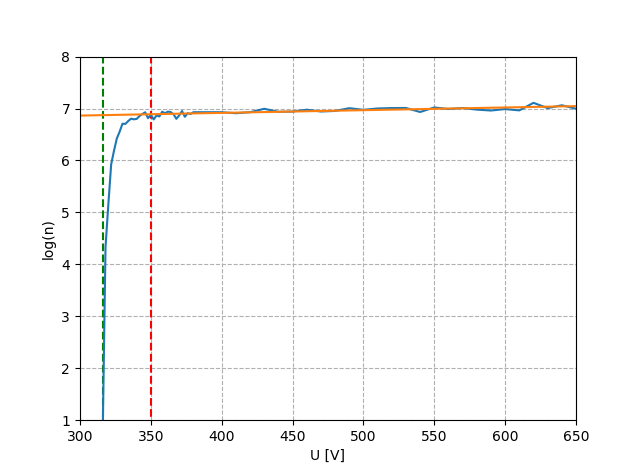
\includegraphics[scale=1]{Bilder/GMlog.PNG}
\caption{Darstellung der Messdaten mitsamt bestimmter Einsatz- und Geigerspannung. Es wurden außerdem die Anpassungen und der Fehlerbereich der Geigerspannung angegeben.}
\label{fig:GMCharakteristik}
\end{figure}
\newpage
\subsubsection{Zusammenfassung}

\begin{table}
\center
\begin{tabular}{|c||c|c|}
\hline 
Methode & Wert &  \\ 
\hline 
Stever & Totzeit$[\mu s]$ & $220\pm 9$ \\ 
\hline 
Stever & Erholungszeit$[\mu s]$ & $469\pm 31$ \\ 
\hline 
Totzeitstufe & Auslösezeit$[\mu s]$ & $318\pm 56$ \\ 
\hline 
Charakteristik & Geigerspannung$[V]$ & $346_{-5}^{+7}$ \\ 
\hline 
Charakteristik & Einsatzspannung$[V]$ & $316.0\pm 0.3$\\ 
\hline 
\end{tabular} 
\caption{Übersicht aller Messergebnisse zum Geiger-Müller-Zählrohr. Es ist zusätzlich die Methode angegeben, mit welcher der entsprechende Wert bestimmt wurde.}
\label{GMzusammenfassung}
\end{table}

In Tabelle \ref{GMzusammenfassung} sind nochmal alle Ergebnisse aufgelistet, die mit dem Geiger-Müller-Zählrohr ermittelt wurden.\\
Wie erwartet liegt die Auslösezeit zwischen der Totzeit und der Erholungszeit. Alle 3 Zeiten liegen in der Größenordnung von$100\mu s$, was wegen der Funktionsweise eines solchen Zährohrs erwartet wurde\footnote{Quelle: https://de.wikipedia.org/wiki/Zählrohr}. Die relativen Fehler sind mit 4-18\% wegen den verwendeten Methoden relativ groß, dies hat aber nur einen geringen Einfluss auf weitere Auswertungen, weswegen diese Fehler akzeptabel sind.\\
\\
Die Charakteristik des Zählrohres konnte außerdem auf 2\% genau bestimmt werden. Der optimale Bereich der Einsatzspannung bildet dabei ein Plateau, das eine Steigung von weniger als 2\% in der logarythmischen Darstellung hat. 

\newpage
\subsection{Proportionalzähler}

\subsubsection{Charakteristik}


\begin{figure}
\centering
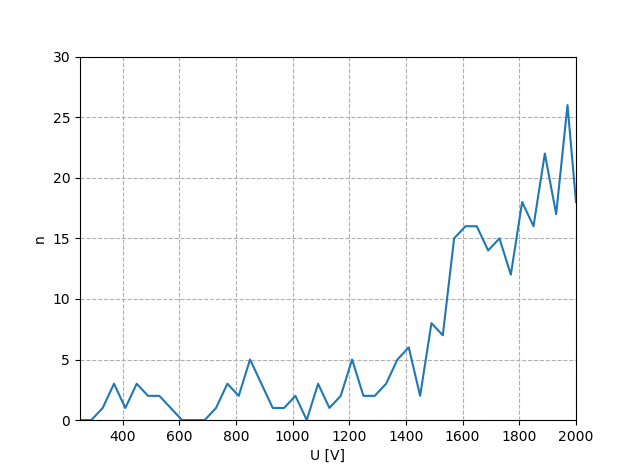
\includegraphics[scale=0.8]{Bilder/Prop/leer.PNG}
\caption{Ergebnis der Leermessung.}
\label{fig:leer}
\end{figure}

\begin{figure}
\centering
\includegraphics[scale=0.8]{Bilder/Prop/Am_lin.PNG}
\includegraphics[scale=0.8]{Bilder/Prop/Am_log.PNG}
\caption{Ergebnisse der Zählratenmessung mithilfe von Americium. Aufgetragen ist die gesamte Zählrate gegen die Spannung. \textbf{Oben}: Darstellung der Rohdaten. \textbf{Unten}: Logarythmisierte Daten mit der Anpassung an das Plateau.}
\label{fig:amlin}
\end{figure}
\begin{figure}
\centering
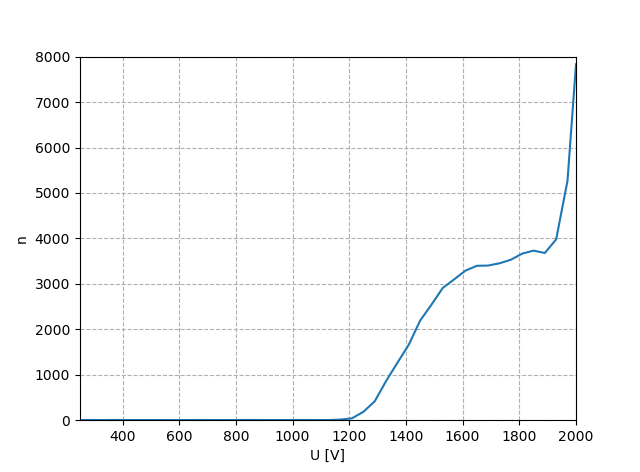
\includegraphics[scale=0.8]{Bilder/Prop/C_lin.PNG}
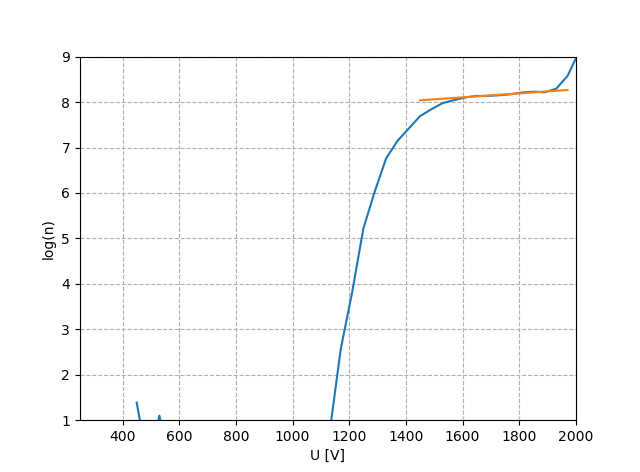
\includegraphics[scale=0.8]{Bilder/Prop/C_log.PNG}
\caption{Ergebnisse der Zählratenmessung mithilfe von Kohlenstoff. Aufgetragen ist die gesamte Zählrate gegen die Spannung. \textbf{Oben}: Darstellung der Rohdaten. \textbf{Unten}: Logarythmisierte Daten mit der Anpassung an das Plateau}
\label{fig:clin}
\end{figure}

Die Pulsraten für das Americium-Präparates sind in Abbildung  \ref{fig:amlin} dargestellt und die des Kohlenstoff-Präparates in Abbildung \ref{fig:clin}. Dabei wurden die Daten aus dem gleichen Grund wie beim Geiger-Müller-Zählrohr logarythmisiert (vgl. Kapitel \ref{GMchar}).\\
\paragraph{Leermessung}
Es wurde außerdem eine Leermessung durchgeführt. Diese ist in Abbildung \ref{fig:leer} zu sehen. Die Zählrate des Hintergrundrauschen ist scheinbar exponentiell. Sie nimmt also mit steigender Spannung immer weiter zu.\\
Dies liegt daran, dass das Zählrohr bei steigender Spannung empfindlich auf Teilchen mit kleineren Energien wird, wodurch auch diese Teilchen einen Puls auslösen können. Außerdem werden immer mehr Selbstentladungen gemessen.

\paragraph{C-Präparat}
$_6^{14} C$ ist ein $\beta$-Strahler. Aus diesem Grund ist wie erwartet nur das Plateau in den Daten zu sehen, in das sowohl $\alpha$ als auch $\beta$ Strahlung mit einfließen.\\
Um die Breite des Plateaus abschätzen zu können wurde ein Linearer fit an die logarythmisierten Werte angepasst und abgeschätzt, welche gemessenen Spannungswerte  mit dieser Anpassung übereinstimmt. Die Anpassung ist in Abbildung \ref{fig:CPlateau} dargestellt. Offensichtlich beginnt das Plateau bei $\SI{1570\pm 12}{V}$ und geht bis $\SI{1930\pm 12}{V}$. Aus dem Fit ergibt sich außerdem eine Steigung von $a = (5.7\pm0.3)\cdot 10^{-4}$. Dies entspricht einer Zunahme der logarythmischen Zählrate von 0.6\% pro 100V.
\begin{figure}
\centering
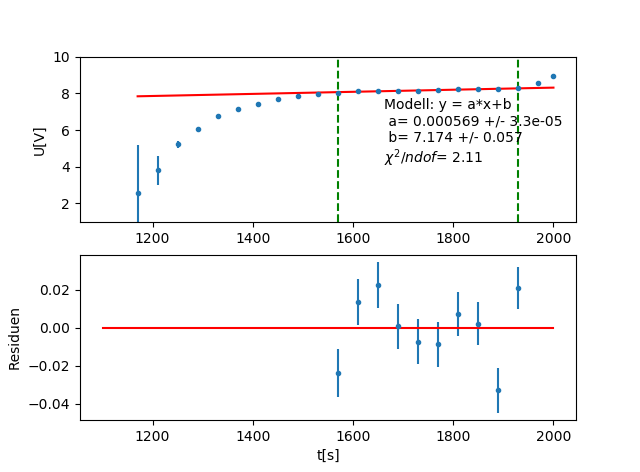
\includegraphics[scale=0.8]{Bilder/Prop/C_plateau.PNG}
\caption{Anpassung einer Gerade and das Plateau in der Charakteristik, die mit dem C-Präparat aufgenommen wurde. Die senkrechten Linien beschreiben den Bereich, der für die Anpassung benutzt wurde.}
\label{fig:CPlateau}
\end{figure}\\
\\
Erst ab einer Spannung von $\SI{1130\pm 12}{V}$ werden überhaupt nennenswerte Pulsraten gemessen. Anscheinend wird ab dieser Spannung also $\beta$-Strahlung gemessen, dass $\alpha$-Plateau hört also vermutlich bei dieser Spannung auf.\\
Auffällig ist, dass die Leermessung bei einer ähnlichen Spannung anfängt zu steigen. Das Zählrohr wird also ab dieser Spannung wesentlich empfindlicher, was sich auf die Zunahme der Zählrate innerhalb des Plateaus auswirkt.

\paragraph{AM-Präparat}
Armericium ist sowohl ein $\alpha$-, als auch ein $\beta$-Strahler. Theoretisch sollten also beide Plateaus in der Messung zur Pulsrate sichtbar sein. Im den Daten ist aber nur ein Plateau sichtbar. Dieses wird genau so wie das Plateau des C-Präparates abgeschätzt, was in Abbildung \ref{fig:AMPlateau} zu sehen ist.

\begin{figure}
\centering
\includegraphics[scale=0.8]{Bilder/Prop/Am_plateau.PNG}
\caption{Anpassung einer Gerade an das Plateau der Am-Charakteristik. Auch hier wird mit den senkrechten Linien der Anpassungsbereich gekennzeichnet}
\label{fig:AMPlateau}
\end{figure}

Das Plateau befindet sich in einem Spannungsbereich von $\SI{760\pm 6}{V}$ bis $\SI{1180\pm 6}{V}$ und hat eine Steigung von $a = (8.6\pm1.4)\cdot 10^{-5}$. Die Zählrate steigt also um weniger als $0.1\%$ pro 100V.\\
 Das Plateauende ist mit dem Ergebnis der C-Proben Auswertung verträglich, bei dem die Zählung von $\beta$-Strahlung bei c.a 1130V einsetzt. Im Bereich bis 1180V ist die Zunahme der Zählrate durch diese Strahlung so klein, dass man sie nicht aus der Messstreuung herausfiltern kann.\\
Direkt nach diesem Plateau gibt es einen kleines zweites Plateau zwischen 1300V und 1400V. Es handelt sich hier wahrscheinlich einfach um eine Messungenauigkeit, da kurz vor dieser Spannung die Verstärkung der Hochspannungsquelle umgeschaltet wurde.\\
\\
Das zweite Plateau, welches nach den Ergenissen von der C-Probe bei c.a 1570V anfangen sollte, fehlt in diesen Messdaten. Die Zählrate steigt zwar wie erwartet durch die $\beta$-Strahlung um ein vielfaches von c.a 15000 auf über 115000 an, statt aber ein 2. Plateau zu bilden, fängt sie bei sehr hohen Spannungen wieder an zu fallen.\\
Dieser Effekt ist unerwünscht und kann viele Ursachen haben.\\
Ein Grund dafür kann sein, dass bei zu hohen Spannungen das zu viel Gasverstärkung stattfindet, wodurch das Zählrohr wie ein Geiger Müller Zählrohr blockiert und somit eine größere Totzeit besitzt.\\
Es kann aber auch sein, dass Fremdatome, die sich in das Gas mischen, den Ionisationsprozess beeinflussen und bei hohen Spannungen das Zählrohr aus unbekannten Gründen blockieren.\\
Ein anderer Grund kann sein, dass bei diesen hohen Spannungen zu viele Pulse gemessen werden und der Verstärker oder das Zählgerät diese nicht mehr auflösen kann, wodurch mehrere Pulse als einer gezählt werden.\\
\\
Die Einsatzspannung ist hier wesentlich kleiner als bei der C-Probe und liegt außerhalb der unseres Messbereiches. Dies liegt daran, dass die durch die Americium-Zerfallsreihe entstehende $\alpha$-Strahlung eine Energie besitzt, die 
um ungefähr ein zehnfaches größer ist als die $\beta$-Strahlung der C-Probe. Dadurch finden schon bei niedrigen Spannungen genug Inonisationsprozesse statt, um einen Messpuls auszulösen.\\


\subsubsection{Pulshöhen}

Die durch die Gasverstärkung erzeugte Anzahl an Elektron-Ion-Paaren aus einem einzelnen Paar ist exponentiell, da jedes erzeugte Paar wieder eine neues Paar erzeugen kann. Aus einem einzelnen Elektron werden also nach einem Verstärkungsschritt (im Mittel) 2, nach 2 Schritten 4, nach 3 Schritten 8 und so weiter.\\
Da mit der angelegten Spannung auch die Anzahl der durchschnittlichen Verstärkungsschritte, die ein Elektron auslöst, zunimmt, wird somit erwartet, dass die gemessene Pulsstärke exponentiell mit der Spannung ansteigt.\\
Deswegen wurden die Pulshöhen logarythmisiert, da in dieser Darstellung ein linearer Zusammenhang erwartet wird.\\
\\
Die Pulshöhen sind außerdem nicht alle gleich groß. Dies liegt daran, dass die Teilchen nicht alle im gleichen Abstand vom Zähldraht und auch nicht alle die gleiche Länge des Rohres durchfliegen. Dadurch kann die Pulshöhe für Teilchen mit gleicher Energie teilweise stark variieren, was das Ablesen am Oszilloskop sehr ungenau macht.\\
Der Ablesefehler kann wegen der Ablesemethode nur qualitativ abgeschätzt werden und ist wegen der Schwankung der Höhen relativ groß. Es wurde allgemein angenommen, dass der Fehler $10\%$ des Wertes beträgt.

\begin{figure}
\centering
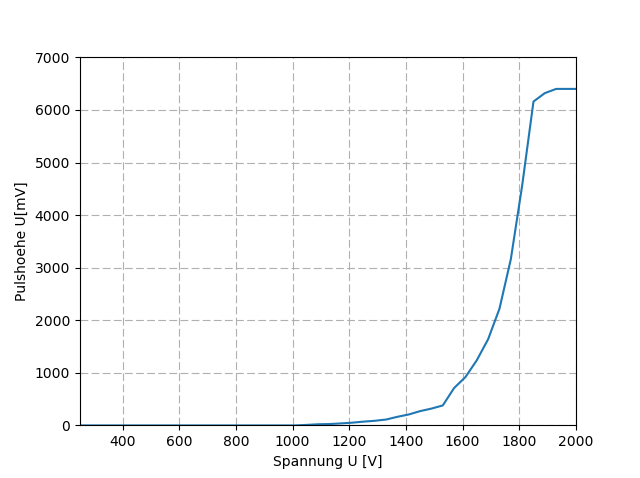
\includegraphics[scale=0.8]{Bilder/Prop/C_Puls_lin.PNG}
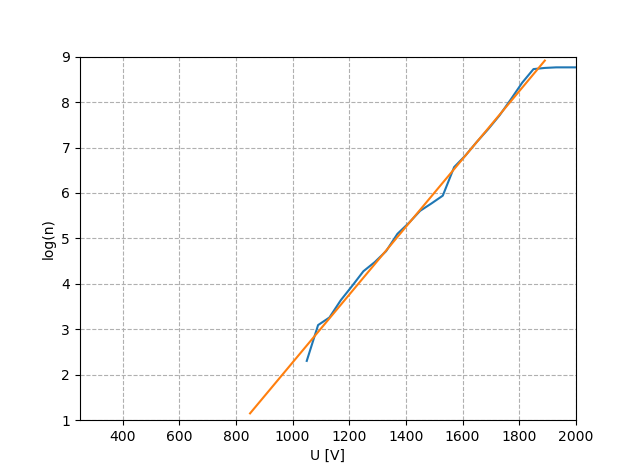
\includegraphics[scale=0.8]{Bilder/Prop/C_Puls_exp.PNG}
\caption{Pulshöhe des C-Präparates in Abhängigkeit von der Spannung. \textbf{Oben}: Rohdaten. \textbf{Unten}: logarythmisierte Daten mit einem Geradenfit an den Linearen Bereich.}
\label{fig:CPulse}
\end{figure}

\begin{figure}
\centering
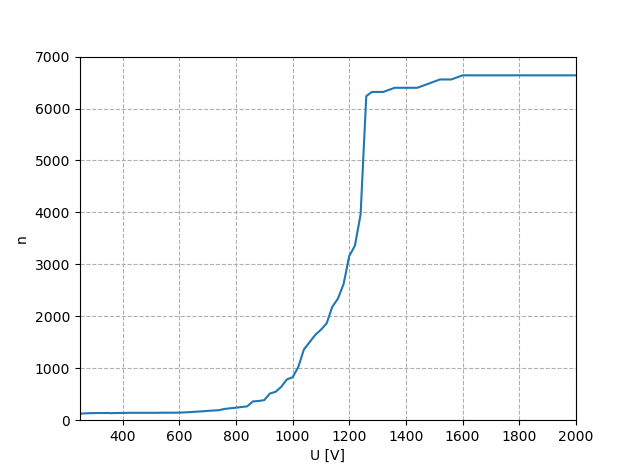
\includegraphics[scale=0.8]{Bilder/Prop/Am_Puls_lin.PNG}
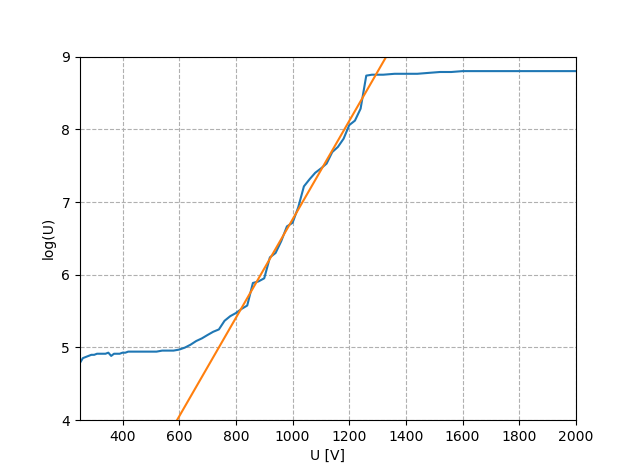
\includegraphics[scale=0.8]{Bilder/Prop/Am_Puls_exp.PNG}
\caption{Pulshöhe des AM-Präparates in Abhängigkeit von der Spannung. \textbf{Oben}: Rohdaten. \textbf{Unten}: logarythmisierte Daten mit einem Geradenfit an den Linearen Bereich.}
\label{fig:AMPulse}
\end{figure}

\paragraph{C-Probe}
Die Abhängigkeit der Pulshöhen von der angelegten Spannung für die C-Probe ist in Abbildung \ref{fig:CPulse} dargestellt.\\
Da bei dieser Probe erst bei Spannungen von c.a 1100V eine von der Hintergrundstrahlung abweichende Zählrate gemessen wird, kann auch erst ab einer ähnlichen Spannung die Pulshöhe bestimmt werden.\\
Bei einer gemessenen Pulshöhe von $\SI{6400}{mV}$ wird eine Maximalspannung erreicht, wodurch das exponentielle Verhalten abbricht und die Pulshöhe nicht mehr weiter ansteigt. Dies ist vermutlich eine Limitierung durch den Aufbau. Enteder ist dies die maximale Spannung, die vom Oszilloskop angezeigt werden kann, oder die maximal erreichbare Verstärkung. Andererseits kann es auch sein, dass bei dieser Pulshöhe eine Sättigung des Proportionalzählers auftritt, wodurch die Anzahl der erzeugten Elektronen nicht mehr weiter ansteigen kann.\\
\\
An den linearen Teil der Daten in der logarythmischen Darstellung wird nun eine Gerade angepasst, um den Zusammenhang zwischen Pulshöhe und Spannung genauer untersuchen zu können. Dieser Fit ist in Abbildung \ref{fig:CPulsfit} dargestellt.\\

\begin{figure}
\centering
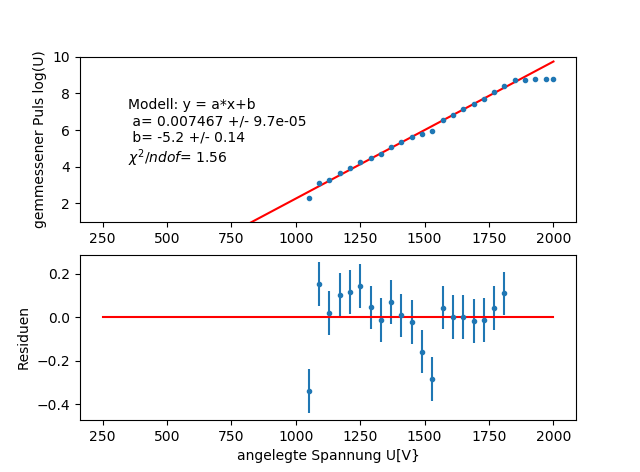
\includegraphics[scale=0.8]{Bilder/Prop/C_Pulsfit.PNG}
\caption{Geradenfit das den Linearen Bereich der Pulshöhe des C-Präparates.}
\label{fig:CPulsfit}
\end{figure}

Der Zusammenhang ist in einem Bereich von 1050V bis 1810V linear. Dies entspricht dem gesamten Bereich, der durch die oben beschrieben Effekte eingeschränkt wird.\\
Die Steigung in diesem Bereich beträgt $0.0075\pm 0.0001$.

\paragraph{Am-Probe}
Bei der Messung anhand der AM-Probe entstand der gleiche Sättigungseffekt, wie bei der C-Probe. Allerdings findet diese Sättigung deutlich früher, bei c.a 1260V, statt. Dies liegt daran, dass die ausgestrahlten $\alpha$-Teilchen eine deutlich größere Energie besitzen und deswegen auch einen größeren Puls erzeugen.\\
Die Einsatzspannung liegt wieder außerhalb des Messbereiches.\\
Auch hier wurde wieder ein linearer Fit einem geeigneten Datenbereich angepasst. Dazu wurde ein Bereich zwischen 900V und 1240V ausgewählt, für den die Daten linear erscheinen. Dies ist in Abbildung \ref{fig:AMPulsfit} dargestellt.\\
Nach diesem Fit konnte der Lineare Zusammenhang für eine Spannung zwischen $\SI{800\pm 6}{V}$ und $\SI{1300\pm 12}{V}$ bestätigt werden. Bei kleineren Spannungen befindet man sich offensichtlich noch nicht im Proportionalbereich. Bei größeren Spannungen tritt der Sättigungseffekt ein.\\
Die Steigung beträgt hier $0.0068\pm 0.0002$, sie ist also etwas kleiner als beim C-Präparat. Dies ist nicht verwunderlich, da hier im relevanten Bereich hauptsächlich $\alpha$-Strahlung gemessen wird. Diese hat eine wesentlich größere Ionisationswahrscheinlichkeit, wodurch bereits sehr viele Elektronen im Strahlengang erzeugt werden und deswegen durch höhere Spannungen nicht die relative Anzahl nicht so stark zunimmt.



\begin{figure}
\centering
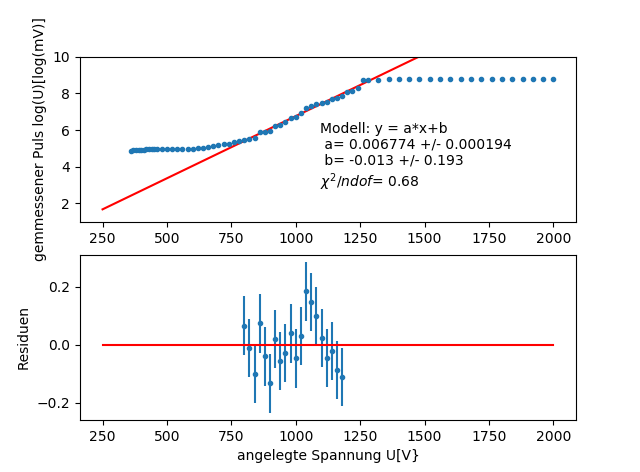
\includegraphics[scale=0.8]{Bilder/Prop/AM_Pulsfit.PNG}
\caption{Geradenfit an den linearen Bereich des Am-Präparates.}
\label{fig:AMPulsfit}
\end{figure}
\newpage
\subsubsection{Zusammenfassung}
In der Charakteristik konnte bei dem AM-Präparat nur das $\alpha$-Plateau identifiziert werden. Dieses liegt in einem Spannungsbereich von $\SI{760\pm 6}{V}$ bis $\SI{1180\pm 6}{V}$. Beim C-Präparat konnte wie erwartet nur das 2.Plateau identifiziert werden, welches im Spannungsbereich von $\SI{1570\pm 12}{V}$ bis $\SI{1930\pm 12}{V}$ liegt. Die Steigungen dieser Plateaus liegen im Promille-Bereich.\\
\\
Die Einsatzspannung liegt beim C-Präparat (und damit für $\beta$-Strahlung) wesentlich höher als beim Am-Präparat, bei welchem auch $\alpha$-Strahlung gemessen wird.\\
\\
In den Pulsraten konnte bei beiden Proben ein linearer Zusammenhang in der logarythmischen Darstellung festgestellt werden. Die Steigungen sind allerdings wegen unterschiedlicher gemessener Teilchen leicht unterschiedlich. Der Proportionalbereich beginnt außerdem erst bei $(800\pm6)V$.
\newpage


\subsection{Statistikmessung}

\subsubsection{Poissonverteilung}
\begin{figure}
\centering
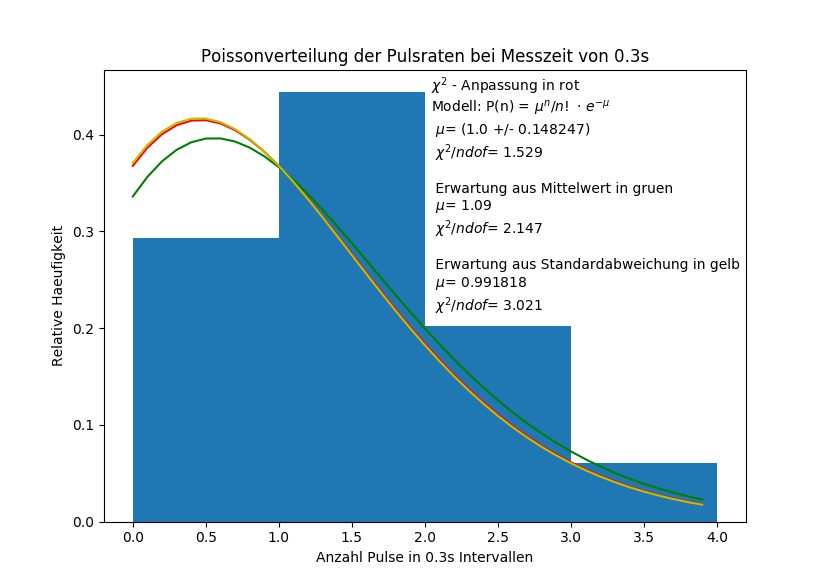
\includegraphics[scale=0.8]{Bilder/poisson.PNG}
\caption{Darstellung der gemessenen Poissonverteilung mit den Erwartungen und der Anpassung.}
\label{fig:Poisson}
\end{figure}

\begin{table}
\centering
\begin{tabular}{|c|c|c|c|}
\hline 
Art & Poisson Parameter & $\chi ^2$ /ndof & P($\chi ^2$) \\ 
\hline 
Mittelwertbestimmung & 1,0900 & 2.147 & 15\% \\ 
\hline 
Bestimmung der Standardabweichung & 0,9918 & 3,021 & 7\% \\ 
\hline 
$\chi ^2$ Anpassung & 1,000 $\pm$ 0,1482 & 1,529 & 28\% \\ 
\hline 
\end{tabular} 
\caption{Poisson Parameter und $\chi ^2$ aus den verschiedenen Bestimmungsmethoden der Poissonverteilung. In der letzten Spalte ist eine geschätzte Wahrscheinlichkeit für den Wert des $\chi ^2$ angegeben.}
\label{tab:Poisson}
\end{table}

Für die Poissonverteilung wird die Anzahl der Pulse im Geiger-Müller-Zählrohr für ein festgelegtes Messintervall wiederholt gemessen. Die auftretenden Anzahlen werden dann in Intervalle mit Breite 1 zusammengefasst und aufgetragen. Das Ergebnis zeigt das Histogramm in Abbildung \ref{fig:Poisson} zusammen mit der $\chi ^2$ Anpassung (in rot) und den Erwartungen die sich aus der Bestimmung des Mittelwertes (grün) und der Standardabweichung (gelb) ergeben.\\
Für die Anpassung wurde auf jeden Wert ein Fehler gemäß der Poissonverteilung angenommen:
\begin{equation*}
\sigma _{n} = \sqrt{n}
\end{equation*}
Für die Anpassung einer Poissonverteilung wurden die Werte normiert, daher pflanzt sich der Fehler fort zu:
\begin{equation*}
n_{i, norm} = \dfrac{n_i}{\sum _j n_j} =: \dfrac{n_i}{N}
\end{equation*}
\begin{equation*}
\sigma _{i, norm} = \sqrt{ \sum _j \left( \sigma_j \cdot \left( \delta_{ij} \cdot \left( \frac{1}{N} - \frac{n_i}{N} \right) + (1 - \delta_{ij}) \cdot \frac{n_i}{N^2} \right) \right)^2 }
\end{equation*}
Tabelle \ref{tab:Poisson} zeigt die Ergebnisse aus den verschiedenen Methoden zur Bestimmung des Poisson Parameters und des $\chi ^2$. Leicht lässt sich ersehen, dass die Werte für den Poisson Parameter nah beieinander liegen, insbesondere liegen die Werte aus Bestimmung von Mittelwert und Standardabweichung innerhalb des Fehlers auf den Wert aus der $\chi ^2$ Anpassung.\\
Die $\chi ^2$ pro Freiheitsgrad bei Bestimmung von Mittelwert und Standardabweichung liegen erwartungsgemäß etwas höher als das aus der Anpassung und dennoch beide noch in einem Bereich mit nicht vernachlässigbarer Wahrscheinlichkeit.


\subsubsection{Gaußverteilung}
\begin{figure}
\centering
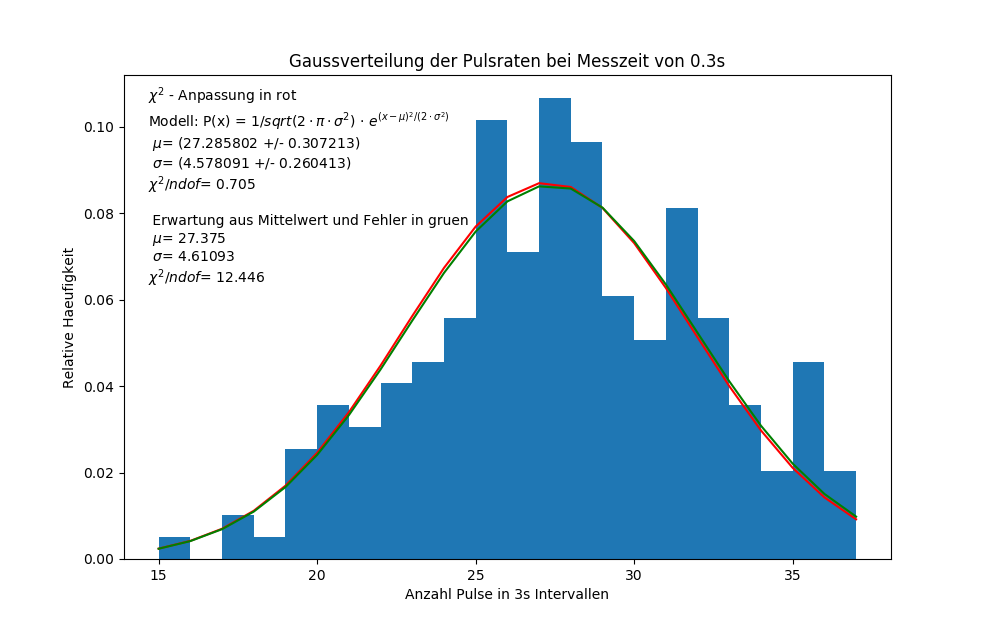
\includegraphics[scale=0.8]{Bilder/gauss.PNG}
\caption{Darstellung der gemessenen Gaußverteilung mit der Erwartung und der Anpassung.}
\label{fig:gauss}
\end{figure}

\begin{table}
\centering
\begin{tabular}{|c|c|c|c|c|}
\hline 
Art & Mittelwert & Standardabweichung & $\chi ^2$ /ndof & P($\chi ^2$) \\ 
\hline 
Bestimmung von $\sigma$ und $\mu$ & 27,375 & 4,611 & 0,688 & 30\% \\ 
\hline 
$\chi ^2$ Anpassung & 27,286 $\pm$ 0,307 & 4,578 $\pm$ 0,260 & 0,705 & 30\% \\ 
\hline 
\end{tabular} 
\caption{Mittelwert, Standardabweichung und $\chi ^2$ aus den verschiedenen Bestimmungsmethoden der Gaußverteilung. In der letzten Spalte ist eine geschätzte Wahrscheinlichkeit für den Wert des $\chi ^2$ angegeben.}
\label{tab:Gauss}
\end{table}

Das Verfahren bei der Gaußverteilung ist identisch zu dem Verfahren bei der Poissonverteilung. Es wurde auch die gleiche Fehlerabschätzung verwendet. Abbildung \ref{fig:gauss} zeigt das Ergebnis. Hier ist in rot die $\chi ^2$ Anpassung und die Erwartung aus Mittelwert und Standardabweichung in grün. In diesem Fall gibt es nur eine Erwartung, weil für die Bestimmung der Gaußverteilung Mittelwert und Standardabweichung notwendig sind.\\
Tabelle \ref{tab:Gauss} zeigt die Werte für Mittelwert, Standardabweichung und $\chi ^2$, die sich aus dem Fit und aus der Erwartung durch Bestimmung von Standardabweichung und Mittelwert ergibt. Die Werte für Mittelwert und Standardabweichung stimmen sehr gut überein und die $\chi ^2$ liegen ebenfalls sehr nah beieinander. Die Wahrscheinlichkeit für ein $\chi ^2$ pro Freiheitsgrad von 0,7 liegt ungefähr bei 30\%, daher kann von einer guten Messung gesprochen werden.


\subsubsection{Exponentialverteilung}
\begin{figure}
\centering
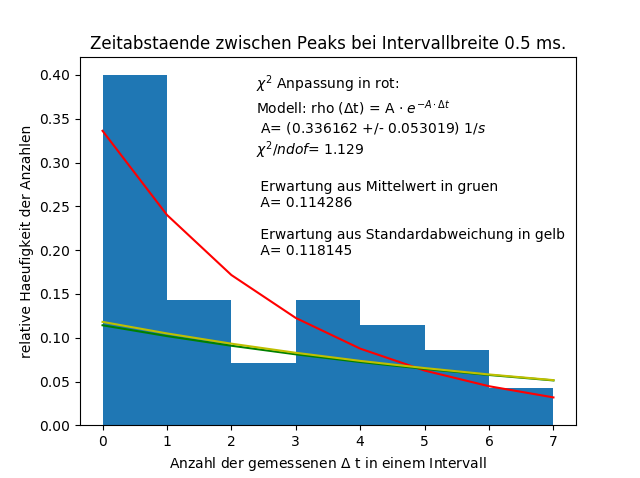
\includegraphics[scale=0.8]{Bilder/Peakabstaende.PNG}
\caption{Darstellung der gemessenen Peakabstände mit den Erwartungen und der Anpassung.}
\label{fig:exponential}
\end{figure}

\begin{table}
\centering
\begin{tabular}{|c|c|c|c|}
\hline 
Art & Exponentialparameter & $\chi ^2$ /ndof & P($\chi ^2$) \\ 
\hline 
Bestimmung von $\mu$ & 0,1143 & 11,307 & 0\% \\ 
\hline 
Bestimmung von $\sigma$ & 0,1181 & 11,302 & 0\% \\ 
\hline 
$\chi ^2$ Anpassung & 0,3362 $\pm$ 0,053 & 1,129 & 22\% \\ 
\hline 
\end{tabular} 
\caption{Exponential Parameter und $\chi ^2$ aus den verschiedenen Bestimmungsmethoden der Exponentialverteilung. In der letzten Spalte ist eine geschätzte Wahrscheinlichkeit für den Wert des $\chi ^2$ angegeben.}
\label{tab:Exponential}
\end{table}

Für die Auswertung der Exponentialverteilung werden die gemessenen Zeitabstände zunächst in sinnvolle Intervalle zusammengefasst. Die Anzahl der gemessenen $\Delta t$, die in diesem Intervall liegen werden auf die x-Achse aufgetragen. Die Anzahl der Intervalle mit der gleichen Anzahl der gemessenen $\Delta t$ wird auf die y-Achse aufgetragen. Dabei wird wieder normiert, daher kann wieder die gleiche Fehlerabschätzung wie bei der Poissonverteilung verwendet werden. Abbildung \ref{fig:exponential} zeigt das Ergebnis. Hier gibt es wieder zwei Erwartungen aus Bestimmung des Mittelwertes (grün) und Bestimmung der Standardabweichung (gelb). Die $\chi ^2$ Anpassung ist wieder in rot eingezeichnet.\\
Tabelle \ref{tab:Exponential} zeigt die Ergebnisse für den Exponentialparameter und das $\chi ^2$ pro Freiheitsgrad für die verschiedenen Bestimmungsmethoden. Auffällig ist, dass die Exponentialparameter aus den Bestimmungen von Mittelwert und Standardabweichung nah beieinander liegen, der Wert aus der $\chi ^2$ Anpassung jedoch deutlich von diesen abweicht. Das $\chi ^2$ ist bei der Anpassung deutlich besser, als bei den Bestimmungen von Mittelwert und Standardabweichung, sodass davon ausgegangen werden kann, dass der Wert aus der Anpassung näher am echten Wert liegt.

\section{Zusammenfassung}

In der Charakteristik des Geiger Müller Zählrohres konnte das Plateau ab einer Spannung von $(346_{-5}^{+7})\si{V}$ identifiziert werden. Der Einsatzbereich dieses Zählrohrs liegt also zwischen dieser Spannung und der maximal gemessenen Spannung von 650V. Die Einsatzspannung wurde mit $(316.0\pm 0.3) \si{V}$ bestimmt.\\
Der Verlauf der Charakteristik stimmt also mit der Erwartung überein.
\\
Die Totzeit des Zählrohres liegt bei $(220\pm 9) \mu s$, die Auslösezeit bei $(318\pm 56)\mu s$ und die Erholungszeit bei $(469\pm 31)\mu s$. Auch diese Werte stimmen mit einer erwarteten Größenordnung von mehreren $100\mu s$ überein, und die Erwartung, dass die Auslösezeit zwischen Tot- und Erholungszeit liegt, wurde bestätigt.\\
\\
Im Charakteristikverlauf des Proportionalzählers konnten zwar beide Plateaus aus den Messungen mit beiden Proben identifiziert werden, allerdings gab es einen unbekannten Effekt bei der Messung mit dem AM-Präparat, der dazu führte, dass die Zählrate bei hohen Spannungen wieder abgefallen ist und das 2. Plateau deswegen nicht sichtbar ist.\\
Die minimale Spannung, bei der eine Pulsrate gemessen wurde, lag bei der C-Probe mit $(1130\pm 12)V$ deutlich höher als bei der Am-Probe, bei der für alle Spannungen Pulsraten gemessen wurden. Damit wurde bestätigt, dass $\beta$ Strahlung wesentlich schlechter ionisiert und deswegen höhere Betriebspannungen benötigt.\\
\\
In der logarythmisierten Pulshöhe konnte außerdem für beide Präparate ein linearer Zusammenhang festgestellt werden, wobei die Steigung wegen unterschiedlicher wechselwirkenden Teilchen leicht unterschiedlich ist.\\
Mithilfe des AM-Präparates wurde außerdem herausgefunden, dass dieser Proportionalbereich erst bei $(800\pm 6) V$ anfängt.\\
Ab einer gemessenen Spannung von c.a $6.4 mV$ erreicht der Verstärker seine maximale Verstärkung und die Pulshöhe steigt nicht weiter an.






	
\end{document}